% !TEX encoding = UTF-8
%Koma article
\documentclass[fontsize=12pt,paper=letter,twoside]{scrartcl}

%Standard Pre-amble
\usepackage[top=4cm,bottom=4cm,left=3cm,right=3cm,asymmetric]{geometry}
%\geometry{landscape}                % Activate for for rotated page geometry
%\usepackage[parfill]{parskip}    % Begin paragraphs with an empty line rather than an indent
\usepackage[table,xcdraw]{xcolor}
\usepackage{graphicx}

\usepackage{amsmath}
\usepackage{amssymb}
\usepackage{epstopdf}
\DeclareGraphicsRule{.tif}{png}{.png}{`convert #1 `dirname #1`/`basename #1 .tif`.png}
% Listings needs package courier
\usepackage{listings} % Needs 
\usepackage{courier}

\usepackage[framemethod=TikZ]{mdframed}
\usepackage{url}

\usepackage{sty/bsymb} %% Event-B symbols
\usepackage{sty/eventB} %% REQ and ENV
\usepackage{sty/calculation}

%Maths
\usepackage{amssymb,amsmath}
\def\Fl{\mathbb{F}}
\def\Rl{\mathbb{R}}
\def\Nl{\mathbb{N}}
\def\Bl{\mathbb{B}}
\def\St{\mathbb{S}}
\newcommand{\ovr}{\upharpoonright}
\newcommand{\var}[1]{\textit{#1}}
%Useful definitions
\newcommand{\mv}[1]{\textit{m\_#1}}
\newcommand{\cv}[1]{\textit{c\_#1}}
\newcommand{\degree}[1]{^{\circ}\mathrm{#1}}
%\newcommand{\comment}[1]{{\footnotesize \quad\texttt{--}\textrm{#1}}}
\newcommand{\im}[1]{i\texttt{-\!#1}}

\usepackage[headsepline]{scrpage2}
\pagestyle{scrheadings}
\ihead[]{\small EECS4312 Report1}
\ohead[]{\small \thepage}
\cfoot[]{}
\ofoot[]{}


%%%%PVS environment%%%%%%%%%%%%%%%%%%%
\lstnewenvironment{pvs}[1][]
    {\lstset{#1,captionpos=b,language=pvs,
    mathescape=true,
    basicstyle=\small\ttfamily,
    numbers=none,
    frame=single,
    % numberstyle=\tiny\color{gray},
    % backgroundcolor=\color{lightgray},
    firstnumber=auto
    }}
    {}
 %%%%%%%%%%%%%%%%%%%%%%%%%%%%%%%%
 
%%%%Verbatim environment%%%%%%%%%%%%%%%%%%%
\lstnewenvironment{code}[1][]
    {\lstset{#1,captionpos=b,
    mathescape=true,
    basicstyle=\small\ttfamily,
    numbers=none,
    frame=single,
    % numberstyle=\tiny\color{gray},
    % backgroundcolor=\color{lightgray},
    firstnumber=auto
    }}
    {}

% \newenvironment{boxed}[1]
%    {\begin{center}
%    #1\\[1ex]
%    \begin{tabular}{|p{0.9\textwidth}|}
%    \hline\\
%    }
%    { 
%    \\\\\hline
%    \end{tabular} 
%    \end{center}
%    }
 %%%%%%%%%%%%%%%%%%%%%%%%%%%%%%%%
 
 %Text in a box
\newenvironment{textbox}
    {\begin{center}
    \begin{tabular}{|p{0.9\textwidth}|}
    \hline\\
    }
    { 
    \\\\\hline
    \end{tabular} 
    \end{center}
    }

\usepackage{hyperref}

%Highlight \hl{}
\usepackage{soul}

\usepackage{enumitem}
\newlist{mylist}{itemize}{1}
\setlist[mylist]{label=\textbullet,leftmargin=1cm,nosep}

\usepackage{multirow}

% Reduce space between figure and caption
%\usepackage{caption}
%\captionsetup[table]{font=small,skip=0pt}     %% Adjust here
%or equivalently 
\usepackage[font=small,skip=4pt]{caption}

% Set the header
\ihead[]{\small EECS4312 Isolette Assignment}
\title{EECS4312 Isolette Assignment}

%Useful definitions
%\newcommand{\mv}[1]{\textit{m\_#1}}
%\newcommand{\cv}[1]{\textit{c\_#1}}
%\newcommand{\degree}[1]{^{\circ}\mathrm{#1}}
%\newcommand{\comment}[1]{{\footnotesize \quad\texttt{--}\textrm{#1}}}

%%%%%%%%%%%%Enter your names here%%%%%%%%
\author{Drew Noel (cse23217@cse.yorku.ca)
\and{Yuval Alter (cse23163@cse.yorku.ca)}
}
%%%%%%%%%%%%%%%%%%%%%%%%%%%%%%%%

\date{\today} % Display a given date or no date

\begin{document}
\maketitle

\noindent You may work on your own or in a team of no more than two students. \textbf{Submit only one document under one Prism account.}

\bigskip
\noindent \textbf{Prism account used for submission}: cse23217

\bigskip\noindent
Keep track of your revisions in the table below.

\section*{Revisions}

%%%%%%%%%%%%Table of revisions%%%%%%%%
\begin{tabular}{|l|l|p{3in}|}
\hline
Date & Revision& Description \\
\hline
October 29th
& 1.0
& Initial requirements document\\
\hline
\end{tabular}
%%%%%%%%%%%%%%%%%%%%%%%%%%%%%%%%

\newpage

\vspace*{2in}
\begin{center}
\huge{\textbf{Requirements Document}:\\ Temperature control for an Isolette}
\end{center}

\newpage

%%%%%%%%%%%%%%%%%%%%%%%%%%%%%%%
\tableofcontents
\listoffigures
\listoftables
\newpage

%%%%%%%%%%%%%%%%%%%%%%%%%%%%%%%
\section{System Overview}

The System Under Development (SUD) is a computer controller for the thermostat of an Isolette.\footnote{%
The image in Fig~\ref{fig:isolette} is from: \url{www.nufer-medical.ch}.}
An Isolette is an incubator for for an infant that provides controlled temperature, humidity and oxygen (Fig.~\ref{fig:isolette}). Isolettes are used extensively in Neonatal Intensive Care Units for the care of premature infants.

This requirements document is specifically for the control of temperature. The purpose of the Isolette computer controller is to maintain the air temperature of an Isolette within a desired range. It senses the current temperature of the Isolette and turns the heat source on and off to warm the air as needed. If the temperature falls too far below or rises too far above the desired temperature range, it activates an alarm to alert the nurse. The system allows the nurse to set the desired temperature range and to set the alarm temperature range outside the desired temperature range of which the alarm should be activated. This requirements documents follows the specification in \cite{REMH} (Appendix A) except where noted.

\begin{figure}[!htb]
\begin{center}
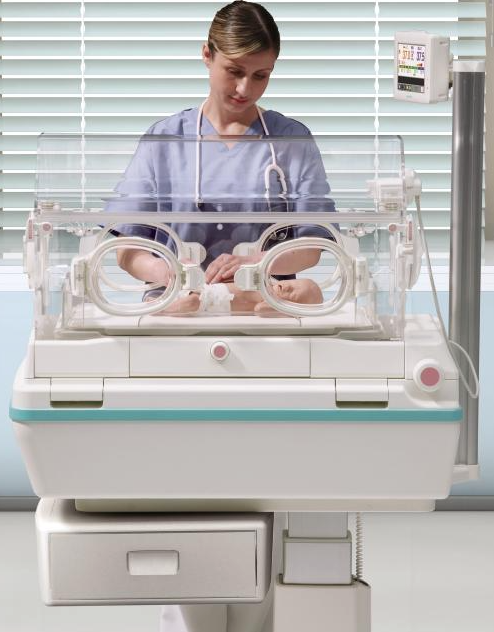
\includegraphics[width=.4\textwidth]{pics/isolette.png}
\end{center}
\caption{Isolette}
\label{fig:isolette}
\end{figure}

%%%%%%%%%%%%%%%%%%%%%%%%%%%%%%%
\section{Context Diagram}

See Fig. A-1 in \cite{REMH}. The System Under Description (SUD) is a computer \emph{controller} to regulate the temperature of the Isolette. Everything else including the Operator Interface (described in \cite{REMH}) is in the ecosystem (i.e. in the environment of the controller). The monitored variables and controlled variables for the controller are in Table~\ref{table:monitored} and
Table~\ref{tbl:cv}, respectively. For clarity, simplicity and safety, there are some differences between the specifications in this document and the descriptions in \cite{REMH}.\footnote{%
Documented in the write-up to this assignment: \texttt{assign1-spec.pdf}.}

%Context Diagram Placed
\begin{figure}[!htb]
\begin{center}
\includegraphics[width=.8\textwidth]{pics/SUD.png}
\end{center}
\caption{SUD Diagram For The Isolette}
\label{fig:isolette_sud}
\end{figure}
%SUD Diagram created using www.draw.io

%%%%%%%%%%%%%%%%%%%%%%%%%%%%%%%
\section{Goals}

The high-level goals (G) of the system are:

\begin{mylist}
\item G1---The Infant should be kept at a safe and comfortable temperature.

\item G2---The Nurse should be warned if the Infant becomes too hot or too cold.

\item G3---The cost of manufacturing the computer controller for the thermostat should be as low as possible.
\end{mylist}

%%%%%%%%%%%%%%%%%%%%%%%%%%%%%%%
\section{Monitored Variables}

The monitored variables are a subset of those described in \cite{REMH}.\footnote{With some change of nomenclature. Monitored variables have an ``m'' prefix.} There is a single status variable \mv{st} that is \emph{invalid} whenever any one of the operator inputs or temperature sensor are in a failed state. Otherwise types and ranges are as in \cite{REMH}.

\begin{table}[h]
\begin{tabular}{|l|l|l|l|l|}
\hline
\cellcolor[HTML]{EFEFEF}Name & \cellcolor[HTML]{EFEFEF}Type & \cellcolor[HTML]{EFEFEF}Range              & \cellcolor[HTML]{EFEFEF}Units & \cellcolor[HTML]{EFEFEF}Physical Interpretation                                       \\ \hline
\mv{tm}                      & $\Rl$                        & $68.0 \upto 105.0$       & $\degree{F}$                   & \begin{tabular}[c]{@{}l@{}}actual temperature of Isolette \\ air temperature from sensor\end{tabular} \\ \hline
\mv{dl}                      & $\intg$                      & $97 \upto 99$      & $\degree{F}$                   & \begin{tabular}[c]{@{}l@{}}desired lower temperature\\ set by operator\end{tabular}   \\ \hline
\mv{dh}                      & $\intg$                      & $98 \upto 100$      & $\degree{F}$                   & \begin{tabular}[c]{@{}l@{}}desired higher temperature\\ set by operator\end{tabular}  \\ \hline
\mv{al}                      & $\intg$                      & $93 \upto 98$      & $\degree{F}$                   & \begin{tabular}[c]{@{}l@{}}lower alarm temperature\\ set by operator\end{tabular}     \\ \hline
\mv{ah}                      & $\intg$                      & $99 \upto 103$      & $\degree{F}$                   & \begin{tabular}[c]{@{}l@{}}higher alarm temperature \\ set by operator\end{tabular}   \\ \hline
\mv{st}                      & Enumerated                   & \{valid, invalid\} &                               & \begin{tabular}[c]{@{}l@{}}status of sensor and \\ operator settings\end{tabular}     \\ \hline
\mv{sw}                      & Enumerated                   & \{on, off\}        &                               & switch set by operator                                                                \\ \hline
\end{tabular}
\caption{Monitored Variables}
\label{table:monitored}
\end{table}

%%%%%%%%%%%%%%%%%%%%%%%%%%%%%%%
\section{Controlled Variables}

The controlled variables are a subset of those described in \cite{REMH}.\footnote{With some change of nomenclature. Controlled variables have a ``c'' prefix.} In addition, there is a mode display \cv{md} and a message display \cv{ms}.\footnote{The mode ``off'' is added to that of Fig.~A-4 in \cite{REMH}, and the mode transitions have been changed.}

\begin{table}[h]
\begin{tabular}{|l|l|l|l|l|}
\hline
\cellcolor[HTML]{EFEFEF}Name & \cellcolor[HTML]{EFEFEF}Type & Range                                                                    & \cellcolor[HTML]{EFEFEF}Units & \cellcolor[HTML]{EFEFEF}Physical Interpretation                                                         \\ \hline
\cv{hc}                      & Enumerated                   & \{on, off\}                                                              &                               & \begin{tabular}[c]{@{}l@{}}heat control: command to\\ turn heat source on or off\end{tabular}           \\ \hline
\cv{td}                      & $\intg$                      & $\{0\} \bunion \{68 \upto 105\}$                                         & $\degree{F}$                  & \begin{tabular}[c]{@{}l@{}}displayed temperature of Isolette\\ (zero when Isolette is off)\end{tabular} \\ \hline
\cv{al}                      & Enumerated                   & \{off, on\}                                                              &                               & sound alarm to call nurse                                                                               \\ \hline
\cv{md}                      & Enumerated                   & \begin{tabular}[c]{@{}l@{}}\{off, init, \\ normal, failed\}\end{tabular} &                               & \begin{tabular}[c]{@{}l@{}}mode of Isolette operation\\ (failed if $\mv{st} = invalid$)\end{tabular}    \\ \hline
\cv{ms}                      & Enumerated                   & \begin{tabular}[c]{@{}l@{}}\{ok, invalid\_sensor, invalid\_alarm\_high, \\ invalid\_alarm\_low\, \\ alarm\_triggered\}\end{tabular} &                               & messages to display to nurse                                                                            \\ \hline
\end{tabular}
\caption {Controlled Variables}
\label{tbl:cv}
\end{table}

%%%%%%%%%%%%%%%%%%%%%%%%%%%%%%%
\section{Mode Diagram}
\hl{To Do}. Provide a statechart for the mode-diagram and provide rationale for the statechart.

%%%%%%%%%%%%%%%%%%%%%%%%%%%%%%%
\section{E/R-descriptions}

% The following requirements were provided in isolette-readme.pdf
\reqm{REQ}
{The \emph{controller} shall operate in one of four modes: \emph{off}, \emph{init}, \emph{normal} and \emph{fail}.\\}
{See statechart in Fig.~\ref{fig:sc}.}
\label{R1}
\textbf{Rationale}: The controller is either: off, awaiting initial valid inputs, in a valid state, or in an invalid state. These are the only possible states, and the transitions are given in Fig.~\ref{fig:sc}.

\reqm{REQ}
{In the \emph{normal} mode, the temperature controller shall maintain current temperature inside the Isolette within a set temperature range (the \emph{desired} range).\\}
{The \emph{desired} temperature range is \emph{m\_dl..m\_dh}. If the current temperature \emph{m\_th} is outside this range, the controller shall turn the heater on or off via the controlled variable \emph{m\_hc} to maintain the desired state.\\}
\label{R2}
\textbf{Rationale}: The \emph{desired temperature range} will be set by the nurse to the desired range based on the infant's weight and health. The controller shall maintain the current temperature within this range under normal operation.

\reqm{REQ}
{In \emph{normal} mode, the controller shall activate an alarm whenever:
\begin{itemize}
    \item the current temperature falls outside the \emph{alarm} temperature range (either through temperature fluctuation or a change in the alarm range by an operator), or
    \item a failure is signalled in any of the input devices (temperature sensor and operator settings).\\
\end{itemize}}
{The alarm temperature range is \emph{m\_al..m\_ah}. Monitored variable \emph{m\_st} shows ``invalid'' when any of the input signals fail.}
\label{R3}
\textbf{Rationale}: The following relevant hazard was identified through the safety assessment process:
\begin{enumerate}
    \item H1: Prolonged exposure of Infant to unsafe heat or cold;
    \item \emph{Classification}: catastrophic
    \item \emph{Probability}: $<10^{-9}$ per hour of operation
\end{enumerate}

\reqm{REQ}
{Once the alarm is activated, it becomes deactivated in one of two ways:
\begin{itemize}
\item The nurse turns off the Isolette
\item The alarm has lasted for 10 seconds, and after 10 seconds or more the alarm conditions are removed. \\
\end{itemize}}
{If the Isolette is powered on, the alarm will sound for 10 seconds, or until the alarm conditions no longer exist, whichever is later.}
\label{R4}
\textbf{Rationale}: Avoid transient alarms, and only turn off the alarm once the conditions that triggered the alarm have been removed.

\reqm{ENV}
{The current temperature received from the sensor is a real number in the range 68.0$\degree{F}$ to 105.0$\degree{F}$.\\}
{The environment assures that the sensor will be in the given range, and it is not required to account for temperatures outside this range.}
\label{E5}
\textbf{Rationale}: The sensor has some given range due to its nature, which allows for restriction of the expected input.

\reqm{ENV}
{The desired and alarm temperatures received from the operator are all in increments of 1$\degree{F}$.\\}
{The inputs for the temperatures will be limited to integers, due to the nature of the environment}
\label{E6}
\textbf{Rationale}: The given inputs have some given granularity, imposed requirements on the SUD.

\hl{TODO: Decide on 3 other E/R descriptions to list}

%%%%%%%%%%%%%%%%%%%%%%%%%%%%%%%
\section{Abstract variables needed for the Function Table}
\hl{If needed, provide abstract variables here. Otherwise, state that abstract variables are not needed.}

\begin{enumerate}
    \item $init\_cond = m\_st(i) = valid \wedge m\_dl(i) <= m\_tm(i) \wedge m\_tm(i) <= m\_dh(i) \wedge m\_al(i) < m\_dl(i) \wedge m\_dl(i) < m\_dh(i) \wedge m\_dh(i) < m\_ah(i)$
    \label{eq:initcond}
\end{enumerate}
%%%%%%%%%%%%%%%%%%%%%%%%%%%%%%%
\section{Function Table}

\subsection{Function Table for heat control: \cv{hc}}
\begin{table}[htb]
\centering
\begin{tabular}{ll|l|}
\cline{3-3}
                                                      &                                                                                & $c\_hc$      \\ \hline
\multicolumn{2}{|l|}{$i=0$}                                                                                                              & off        \\ \hline
\multicolumn{1}{|l|}{\multirow{3}{*}{$i > 0$}} & $m\_tm(i) > m\_dh(i)$                                                 & off        \\ \cline{2-3}
\multicolumn{1}{|l|}{}                                & $m\_tm(i) < m\_dl(i)$                                                    & on         \\ \cline{2-3}
\multicolumn{1}{|l|}{}                                & $m\_tm(i) \le m\_dh(i) \wedge  m\_tm(i) \ge m\_dl(i)$ & $c\_hc(i-1)$ \\ \hline
\end{tabular}
\caption{Function Table for heat control: \cv{hc}}
\end{table}

\subsection{Function Table for displayed temperature: \cv{td}}
\hl{TODO}
\subsection{Function Table for alarm: \cv{al}}
\hl{TODO}
\subsection{Function Table for Isolette mode: \cv{md}}
\begin{table}[htb]
\centering
\begin{tabular}{llll|l|}
\cline{5-5}
                                                        &                                                  &                                                           &                    & $c\_md$  \\ \hline
\multicolumn{4}{|l|}{$i = 0$}                                                                                                                                                                 & off    \\ \hline
\multicolumn{1}{|l|}{\multirow{8}{*}{$i > 0$}} & \multicolumn{3}{l|}{$m\_sw =$ off}                                                                                                  & off    \\ \cline{2-5}
\multicolumn{1}{|l|}{}                                  & \multicolumn{1}{l|}{\multirow{7}{*}{$m\_sw =$ on}} & \multicolumn{2}{l|}{$c\_md(i-1) =$ off}                                          & init   \\ \cline{3-5}
\multicolumn{1}{|l|}{}                                  & \multicolumn{1}{l|}{}                            & \multicolumn{1}{l|}{\multirow{2}{*}{$c\_md(i-1) =$ init}}   & $init\_cond$ \footnotemark        & normal \\ \cline{4-5}
\multicolumn{1}{|l|}{}                                  & \multicolumn{1}{l|}{}                            & \multicolumn{1}{l|}{}                                     & $\neg init\_cond$     & init   \\ \cline{3-5}
\multicolumn{1}{|l|}{}                                  & \multicolumn{1}{l|}{}                            & \multicolumn{1}{l|}{\multirow{2}{*}{$c\_md(i-1) =$ normal}} & $m\_st(i) =$ invalid & failed   \\ \cline{4-5}
\multicolumn{1}{|l|}{}                                  & \multicolumn{1}{l|}{}                            & \multicolumn{1}{l|}{}                                     & $m\_st(i) =$ valid   & normal \\ \cline{3-5}
\multicolumn{1}{|l|}{}                                  & \multicolumn{1}{l|}{}                            & \multicolumn{1}{l|}{\multirow{2}{*}{$c\_md(i-1) =$ failed}}   & $m\_st(i) =$ valid   & normal \\ \cline{4-5}
\multicolumn{1}{|l|}{}                                  & \multicolumn{1}{l|}{}                            & \multicolumn{1}{l|}{}                                     & $m\_st(i) =$ invalid & failed   \\ \hline
\end{tabular}
\caption{Function Table for Isolette mode: \cv{md}}
\end{table}
\footnotetext{Defined in Abstract Variable \ref{eq:initcond}}

\subsection{Function Table for displayed message: \cv{ms}}
\hl{TODO}

%%%%%%%%%%%%%%%%%%%%%%%%%%%%%%%
\section{Validation}
\hl{To be Done.}
Proof of completeness and disjointness and validation of the requirements using PVS.

Include the PVS sources in the appendix to this document but summarize the proofs here.

%%%%%%%%%%%%%%%%%%%%%%%%%%%%%%%
\section{Use Cases}
See Section A2 of \cite{REMH} for some use cases. The use cases need to be adapted to the revised descriptions of the previous sections of this document.

%%%%%%%%%%%%%%%%%%%%%%%%%%%%%%%
\section{Acceptance Tests}
In this section, the use cases have to be converted into precise acceptance tests (using the function table to describe pre/post conditions) to be run when the design and implementation are complete.

%%%%%%%%%%%%%%%%%%%%%%%%%%%%%%%
\section{Traceability}
Matrix to show which acceptance tests passed, and which R-descriptions they checked.

%%%%%%%%%%%%%%%%%%%%%%%%%%%%%%%
\section{Glossary}
The definition of important terms is placed in this section. You are not required to complete this.

%%%%%%%%%%%%%%%%%%%%%%%%%%%%%%%
\bibliographystyle{plain}
\bibliography{ref}
\end{document}
